\section{Proposed solution: KEALLM - Knowledge Embedding Augmented Large Language Model}
\subsection{Architecture}
This architecture, illustrated in Figure \ref{fig:keallm_arch}, seeks to combine the powerful language processing capabilities of a Large Language Model (LLM) with the rich contextual information embedded within a knowledge graph. The primary goal is to leverage both elements for enhanced language comprehension and generation.\\\\
The process begins with a user query $X_q$. This query is simultaneously fed into two distinct pathways. The first pathway involves a standard Embedding Layer, which converts the raw text of the query into language embedding tokens $H_q$. These tokens represent the semantic meaning of the query in a suitable format by the LLM.\\\\
The second pathway leverages the knowledge graph to provide contextual information. We assume that each user query $X_q$ is associated with a corresponding query triplet ($head$, $relation$, ?), representing the knowledge sought by the query. This triplet is used to query the Knowledge Graph Embedding module, which extracts relevant knowledge features $X_{kn}$. These features encapsulate the relationships and entities within the knowledge graph that belong to the user's query. However, these knowledge features exist in a form incompatible with the LLM. To bridge this gap, a Projector module transforms the knowledge features $X_{kn}$ into language embedding tokens $H_{kn}$.\\\\
The outputs from both pathways, the language embedding tokens $H_q$ from the Embedding Layer and the projected knowledge embedding tokens $H_{kn}$ from the Projector, are then concatenated. This concatenation creates a single input vector that encapsulates both the linguistic content of the user query and the relevant contextual knowledge from the knowledge graph.
This enriched input vector is then passed to the LLM component $f_{\phi}(.)$. The LLM, leveraging its internal parameters $\phi$, processes this input and generates the next token $X_a$ in the response sequence.
This architecture's strength lies in its ability to infuse the LLM's language processing with contextual knowledge derived from a knowledge graph. This fusion allows the LLM to access information beyond the immediate query, potentially leading to more accurate, relevant, and informative responses.
\begin{figure}[hbt]
    \centering
    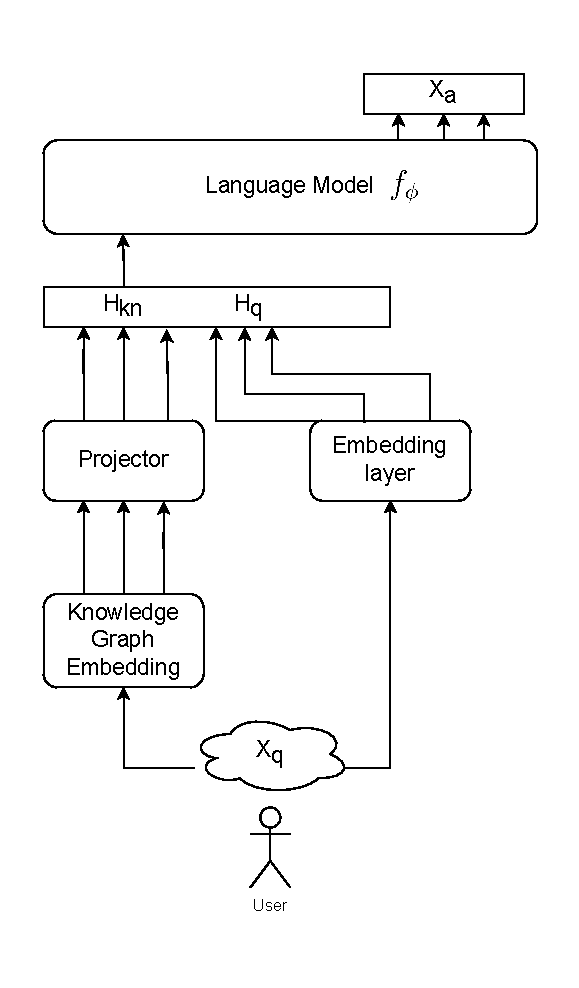
\includegraphics[width=0.6\textwidth]{experiements/image/keallm.pdf}
    \caption{Overall of KEALLM architecture}
    \label{fig:keallm_arch}
\end{figure}

\subsection{Training}
\subsubsection{Pretrained language model knowledge graph embedding module}
This project utilizes a pretrained language model (PLM) based approach for knowledge graph embedding, drawing inspiration from the work presented in KG-BERT\cite{yao2019kg}. This method leverages the power of PLMs to extract and embed knowledge from text, offering a robust and efficient solution for knowledge graph embedding. Each unique entity and relation is treated as a special token within the language model. This approach transforms link prediction into a masked entity prediction problem, building upon the work on $k$-NN KGE\cite{10.1007/978-3-031-44693-1_9}.\\\\
\textbf{Masked Entity Modeling}: A BERT-based model is employed as the entity predictor, converting link prediction into a masked entity modeling task. This approach utilizes structural information and textual descriptions to predict the missing entity in a triple. Given an incomplete triple $(e_i, r_j, ?)$, an input sequence $x_k$ is constructed by concatenating these elements:
\begin{align*}
x_k = \text{\texttt{[CLS]}} e_i \text{\texttt{[SEP}]} r_j \text{\texttt{[SEP]}} \text{\texttt{[MASK]}} \text{\texttt{[SEP]}}
\end{align*}

Through masked entity modeling, the correct entity $e_k$ is identified by ranking the probability of each entity in the knowledge graph based on:

\begin{align}
p(e_k|x_k) = p(\text{\texttt{[MASK]}} = e_k|x_k;\Phi)
\end{align}
where $\Phi$ represents the model's parameters

The model is trained by minimizing the following loss function:
\begin{align}
\mathcal{L}_{kn} = - \mathbb{E}_{(x_k,e_k) \sim \mathcal{D}_{kg}}\log{p(\text{\texttt{[MASK]}} = e_k|x_k;\Phi)}
\end{align}
where $D_{kg}$ is the training set and $\Phi$ represents the parameters of the model.
\begin{algorithm}[hbt]
\caption{Knowledge graph embedding training}\label{alg:kge}
\begin{algorithmic}[1]
\REQUIRE Knowledge graph $G = (E, R, T)$, where $E$ is the set of entities, $R$ is the set of relations, and $T$ is the set of triples.
\REQUIRE Pre-trained language model $\Phi$, e.g., BERT.
\REQUIRE Learning rate $\alpha$, batch size $B$, number of epochs $N$.
\ENSURE Trained model parameters $\Phi$.

\STATE Initialize $\Phi$ with pre-trained weights.
\STATE Expand the vocabulary of $\Phi$ with unique entities in $E$.
\FOR{$epoch = 1$ to $N$}
    \FOR{each batch of triples $(e_i, r_j, e_k) \in T$ of size $B$}
        \STATE Construct input sequence $x_k = \text{\texttt{[CLS]}} e_i \text{\texttt{[SEP}]} r_j \text{\texttt{[SEP]}} \text{\texttt{[MASK]}} \text{\texttt{[SEP]}}$.
        \STATE Obtain probability distribution $p(e|x_k) = p(\text{\texttt{[MASK]}} = e|x_k;\Phi)$ for all entities $e \in E$
        \STATE Calculate the loss $\mathcal{L}_{kn} = - \mathbb{E}_{(x_k,e_k) \sim \mathcal{D}_{kg}}\log{p(\text{\texttt{[MASK]}} = e_k|x_k;\Phi)}$
        \STATE Update model parameters $\Phi$ using a gradient descent optimizer with learning rate $\alpha$ and the loss $\mathcal{L}_{kn}$: $\Phi \leftarrow \Phi - \alpha \nabla_\Phi\matcal{L}$
    \ENDFOR
\ENDFOR

\RETURN $\Phi$
\end{algorithmic}
\end{algorithm}
The process of training knowledge graph embedding is summarized in Algorithm \ref{alg:kge}. After training the knowledge graph embedding model, the feature vectors from the final hidden layer are used as the knowledge features.

\subsubsection{Supervised Fine-Tuning}
The supervised fine-tuning phase focuses on bridging the gap between the structured knowledge encoded in the knowledge graph embeddings and the linguistic understanding of the Large Language Model (LLM). This alignment is accomplished through a dedicated Projector module, which learns to translate knowledge embeddings into a format readily interpretable by the LLM.
The Projector module acts as a bridge between the two worlds: knowledge graphs and natural language. It takes the knowledge embedding $X_{kn}$, representing the relevant entities and relationships extracted from the knowledge graph, and transforms it into a format compatible with the LLM. This transformation is achieved through a trainable projection matrix $W$, represented as the parameter $\theta$ in our model.
Specifically, the Projector module aims to maximize the likelihood of the LLM generating the correct target answer sequence $X_a$, given both the knowledge embeddings $X_{kn}$ and the linguistic features of the user query $X_q$. This likelihood is formally defined in Equation \ref{p_likelihood}:
\begin{align}
\label{p_likelihood}
p(X_a|X_{kn},X_q) = \prod_{i=1}^L p(x_i|X_{kn},X_q,X_{a<i};\theta)
\end{align}
where $L$ represents the length of the answer sequence and $p(X_i|X_{kn},X_q,X_{a<i};\theta)$ denotes the probability of generating the i-th token in the answer, conditioned on the knowledge embeddings, user query and model parameters $\theta$.\\\\
To optimize the Projector module, we utilize a supervised learning approach with a dataset $(x, y)$, where $x$ represents a user query aimed at eliciting a missing entity in a knowledge graph triple $(e_i, r_i, ?)$, and $y$ represents the correct target entity $e_k$.
The training process employs a cross-entropy loss function, which measures the discrepancy between the LLM's predicted probability distribution over its vocabulary and the true target entity:
% $$
% \mathcal{L}_{sft} = -\sum_{(X_{kn}, X_q, X_a) \in \mathcal{D}} \sum_{i=1}^{L} \log p(x_i | X_{kn}, X_q, X_{a<i}; \theta)
% $$
\begin{align}
\mathcal{L}_{sft} = - \mathbb{E}_{(X_{kn},X_q,X_a) \sim \mathcal{D}_{sft}}\sum_{i=1}^{L} \log p(x_i | X_{kn}, X_q, X_{a<i}; \theta)
\end{align}

By minimizing this loss function, we effectively fine-tune the Projector module, enabling it to learn an optimal projection matrix $W$. This optimization ensures that the transformed knowledge embeddings align seamlessly with the LLM's internal language model, ultimately enhancing the LLM's capacity to access and utilize external knowledge for improved response generation.

\begin{algorithm}[hbt]
\caption{Supervised fine-tuning of the Projector module}\label{alg:sft}
\begin{algorithmic}[1]
\REQUIRE Dataset $\mathcal{D}$ of (user query $X_q$, knowledge embedding $X_{kn}$, target entity $X_a$) tuples.
\REQUIRE Pre-trained LLM $f_\phi(.)$.
\REQUIRE Initialized Projector module with parameters $\theta$.
\REQUIRE Learning rate $\alpha$, batch size $B$, number of epochs $N$.
\ENSURE Fine-tuned Projector module parameters $\theta$.
\FOR{$epoch = 1$ to $N$}
\FOR{each batch of tuples $(X_{q}, X_{kn}, X_a) \in \mathcal{D}$ of size $B$}
\STATE Compute the concatenated input vector: $[H_q, H_{kn}]$
\STATE Feed the concatenated vector to the LLM: $f_\phi([H_q, H_{kn}])$
\STATE Obtain the LLM's predicted probability distribution over its vocabulary.
\STATE Calculate the loss $\mathcal{L}_{sft} = - \mathbb{E}_{(X_{kn},X_q,X_a) \sim \mathcal{D}_{sft}}\sum_{i=1}^{L} \log p(x_i | X_{kn}, X_q, X_{a<i}; \theta)$.
\STATE Update Projector module parameters $\theta$ using a gradient descent optimizer with learning rate $\alpha$ and the loss $\mathcal{L}_{sft}$: $\theta \leftarrow \theta - \alpha \nabla_\theta \mathcal{L}_{sft}$.
\ENDFOR
\ENDFOR
\RETURN $\theta$
\end{algorithmic}
\end{algorithm}
Algorithm \ref{alg:sft} demonstrates the process of fine-tuning the projector module.
\subsubsection{Direct Preference Optimization}
Direct Preference Optimization (DPO) further fine-tunes KEALLM by aligning its output with user preferences, achieved by training the model to prefer desired responses over undesired ones. We utilize a dataset $D$ constructed from user queries and their corresponding preferred and less preferred responses derived from a combination of ground truth knowledge and the knowledge graph embedding. For each user query $x$, we obtain the ground truth entity as the preferred answer $y_w$, and an entity with the lowest probability from the knowledge graph embedding module as less preferred answers $y_l$.\\\\
The DPO loss function maximizes the difference in log probabilities between these preferred and less preferred responses:
\begin{align}
\mathcal{L}_{DPO} = -\mathbb{E}_{(x, y_w, y_l) \sim D} \log \sigma \left( \beta \log \frac{\pi_{\theta}(y_w | x)}{\pi_{\text{ref}}(y_w | x)} - \beta \log \frac{\pi_{\theta}(y_l | x)}{\pi_{\text{ref}}(y_l | x)} \right)
\end{align}
where $\pi_{\theta}(y | x)$ is the probability of KEALLM generating response $y$ given query $x$ and model parameters of Projector module $\theta$, $\pi_{\text{ref}}(y | x)$ is the probability of a reference model generating response $y$ given query $x$, $\beta$ scales the emphasis on the probability difference, $\sigma(.)$ is the sigmoid function.

Minimizing this loss encourages the model to assign higher probability to preferred responses compared to less preferred ones, relative to the reference model. This encourages KEALLM to generate responses aligned with the knowledge graph embedding's ranking of relevant entities. The process is summarized in Algorithm \ref{alg:dpo}

\begin{algorithm}[hbt]
\caption{Direct Preference Optimization for KEALLM}\label{alg:dpo}
\begin{algorithmic}[1]
\REQUIRE Dataset $D$ of (user query $x$, preferred responses $y_w$, less preferred responses $y_l$) tuples.
\REQUIRE Pre-trained KEALLM with parameters $\theta$.
\REQUIRE Reference model $\pi_{\text{ref}}$.
\REQUIRE Learning rate $\alpha$, batch size $B$, number of epochs $N$.
\ENSURE Fine-tuned KEALLM parameters $\theta$.
\FOR{$epoch = 1$ to $N$}
\FOR{each batch of tuples $(x, y_w, y_l) \in D$ of size $B$}
\STATE Compute KEALLM probabilities: $\pi_\theta(y_w | x)$, $\pi_\theta(y_l | x)$
\STATE Compute reference probabilities: $\pi_{\text{ref}}(y_w | x)$, $\pi_{\text{ref}}(y_l | x)$
\STATE Calculate the DPO loss: $\mathcal{L}_{DPO}$
\STATE Update KEALLM parameters $\theta$ using a gradient descent optimizer with learning rate $\alpha$ and the loss $\mathcal{L}_{DPO}$:
$\theta \leftarrow \theta - \alpha \nabla_\theta \mathcal{L}_{DPO}$
\ENDFOR
\ENDFOR
\RETURN $\theta$
\end{algorithmic}
\end{algorithm}